\section{Results}

\subsection{Messages size}

Hereafter we list the messages peers exchange in Multipong and their
size\footnote{the size shown in the table has to be intended as ``greater or
equal than''}:

\begin{table}[H]
  \centering
  \begin{tabular}{l|c c}
  & \textbf{\textit{Message}} & \textbf{\textit{Size [B]}}  \tabularnewline
            \hline
            \multirow{5}{*}{TCP} & \multicolumn{1}{c}{\texttt{ARE\_YOU\_HOST}} & \multicolumn{1}{c}{60} \\\cline{2-3}
                                 & \multicolumn{1}{c}{\texttt{AVAILABLE}} & \multicolumn{1}{c}{100} \\\cline{2-3}
                                 & \multicolumn{1}{c}{\texttt{CANCEL}} & \multicolumn{1}{c}{56} \\\cline{2-3}
                                 & \multicolumn{1}{c}{\texttt{DISCOVERY}} & \multicolumn{1}{c}{82} \\\cline{2-3}
                                 & \multicolumn{1}{c}{\texttt{JOIN}} & \multicolumn{1}{c}{54} \\\hline
            \multirow{3}{*}{UDP} & \multicolumn{1}{c}{\texttt{KNOWN\_HOSTS}} & \multicolumn{1}{c}{90} \\\cline{2-3}
                                 & \multicolumn{1}{c}{\texttt{STARTING}} & \multicolumn{1}{c}{187} \\\cline{2-3}
                                 & \multicolumn{1}{c}{\texttt{TELL\_IP}} & \multicolumn{1}{c}{57} \\\hline
        \end{tabular}
  \caption{Messages size}
  \label{tab:sizes}
\end{table}

\subsection{Energy and traffic}

The average power consumption and Wi-Fi Direct traffic can be seen in Figure
\ref{fig:energy} and Figure \ref{fig:traffic}.

\begin{figure}[H]
	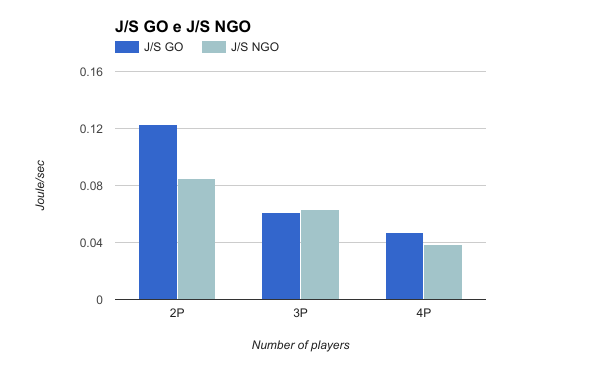
\includegraphics[width=\columnwidth]{img/energy.png}
	
	\caption{GO/NGO comparison for energy}\label{fig:energy}
\end{figure}
%\begin{figure}[H]
%  \centering
%  \begin{tabular}{@{}c@{}c}
%      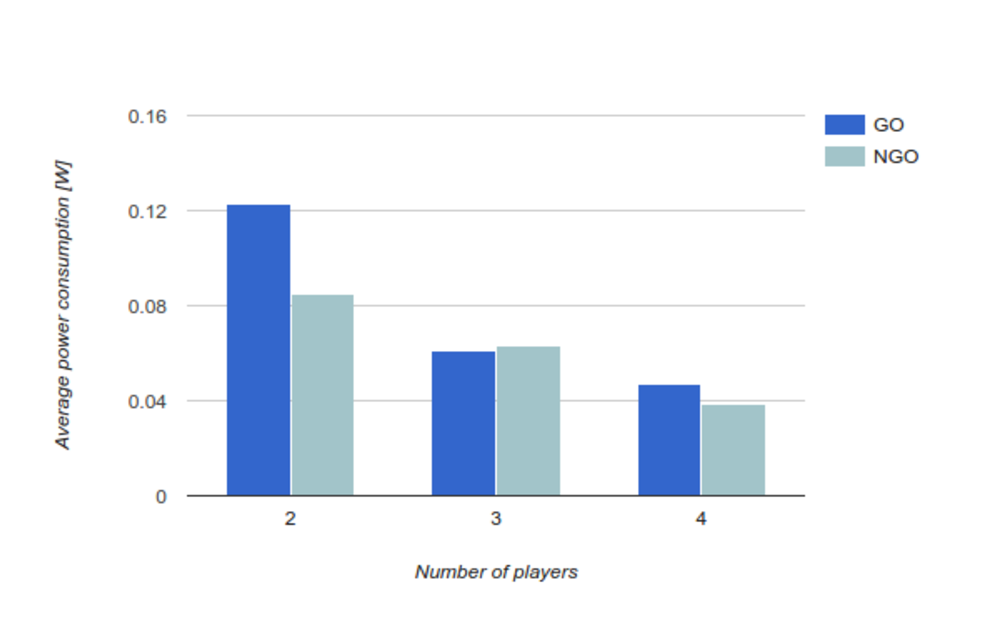
\includegraphics[width=.5\columnwidth]{img/energy.eps}
%      \label{fig:energy}
%    &
%    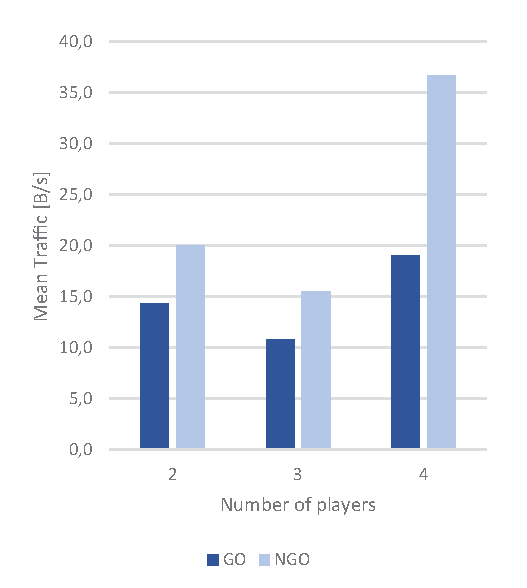
\includegraphics[width=.5\columnwidth]{img/traffic.eps}
%    \label{fig:traffic}
%  \end{tabular}
%  \caption{GO/NGO comparison for energy and traffic}\label{fig:comparison}
%\end{figure}

%%% ENERGY FIGURE

We were able to filter out the bias caused by the human user interaction with
the screen thanks to the autoplay: in fact, in previous tests we found out
that most of the power consumption was caused from moving the palette by hand.

At a first glance, the figure \ref{fig:energy} shows counterintuitive data
because energy consumption happens to be higher with a limited number of
players. However, the plot represents the \textit{average} battery consumption
during the whole session; thus, we think that this is caused by the fact that
the game formation phase is heavier than the gameplay one (which is much longer
in matches with a bigger number of players).

Still, PowerTutor is not a truly reliable tool to measure battery consumption in
our case since we used different devices from the ones used to develop the
PowerTutor's mathematical model. Hence, we can not say too much about how power
consumption varies depending on the number of players. Nonetheless, we noticed
that Multipong is quite light compared to other multimedia applications in
terms of battery consumption.

\begin{figure}[H]
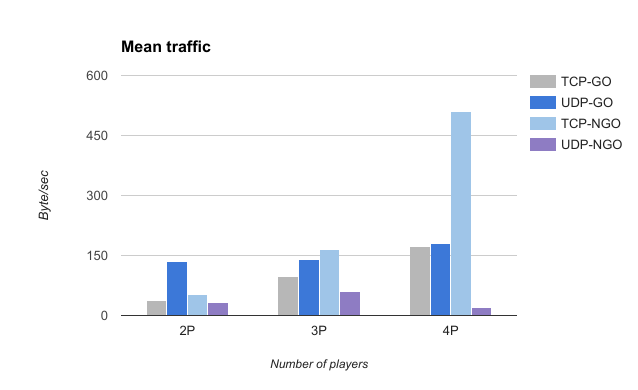
\includegraphics[width=\columnwidth]{img/traffic.png}

\caption{GO/NGO comparison for traffic}\label{fig:traffic}
\end{figure}

%%% TRAFFIC FIGURE

Concerning to the game formation phase, the extent to which traffic grows with
the number of players is striking. On the other hand, during the gameplay phase
the amount of bytes per second is dramatically low since there are significant
dead times (i.e. times where the ball is not in the player's screen) in which
communication is almost null.
It's interesting to notice how much the overhead the GO incurs is limited as
the number of players rises; this fact leads us to suppose that we were not
able to play matches with a high number of players due to the precariousness
of Wi-Fi direct, rather than the overhead caused by the communication among the
peers (which is indeed acceptable for a real-time application).

\subsection{TCP and UDP comparison}

In Figure \ref{fig:TCP-UDP}, we can see the difference between the mean RTTs of
TCP and acked UDP transmissions, which were measured as described in section
\ref{sec:eval-rtt}.

\begin{figure}[H]
  \centering
  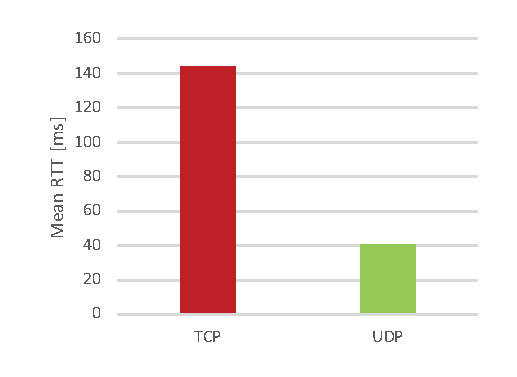
\includegraphics[width=.8\columnwidth]{img/UDPvsTCP-RTT.eps}
  \caption{TCP vs. UDP}
  \label{fig:TCP-UDP}
\end{figure}

As it can be easily seen, acked UDP is very efficient compared to TCP and
therefore we can acknowledge that acked UDP is the most suitable choice (between
these two) in the gameplay phase, whilst TCP is fit for the game formation
phase, when we do not need low latency but more reliable packet delivery.
